\documentclass[12pt]{article}
\usepackage{amsmath}
\usepackage{tikz}
\usepackage{pgfplots}

\pgfplotsset{compat=1.17}

\begin{document}

\title{Understanding\\the Point-Slope Form\\of Linear Equations}\\
\author{Tutoring Centre Ferndale\\

\includegraphics[width=4em]{ApS_logo.png}}
\date{}
\maketitle

In linear algebra, the point-slope form \(y - y_1 = m(x - x_1)\) is useful for writing the equation of a line when the slope \(m\) and a point \((x_1, y_1)\) on the line are known. Understanding how to use and manipulate this form can simplify the process of graphing linear equations and solving related problems.

\section*{Point-Slope Form: \(y - y_1 = m(x - x_1)\)}

In the point-slope form, \(y - y_1 = m(x - x_1)\):
\begin{itemize}
    \item \((x_1, y_1)\) is a point on the line.
    \item \(m\) is the slope of the line.
\end{itemize}

\subsection*{Questions}
\begin{enumerate}
    \item What is the general form of the point-slope equation?
    \item Identify the slope and a point in the equation \(y - 3 = 2(x + 1)\).
    \item How do you derive the point-slope form from a given point and slope?
\end{enumerate}

\newpage

\section*{Graphing Using Point-Slope Form}

To graph a line using the point-slope form:
\begin{itemize}
    \item Plot the point \((x_1, y_1)\) on the coordinate plane.
    \item Use the slope \(m\) to determine the rise and run from the point \((x_1, y_1)\).
    \item Draw the line through the point with the given slope.
\end{itemize}

\subsection*{Example}

Given the equation \(y - 2 = -\frac{1}{2}(x - 4)\):
\begin{itemize}
    \item The point \((4, 2)\) is on the line.
    \item The slope is \(-\frac{1}{2}\).
\end{itemize}

\begin{center}
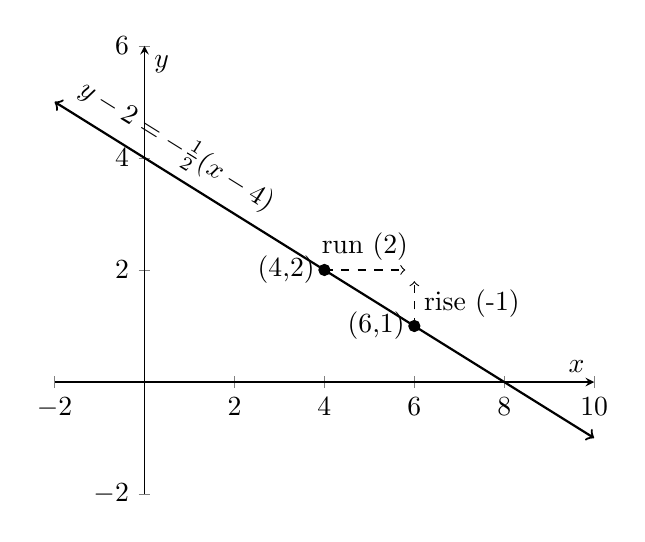
\begin{tikzpicture}
    \begin{axis}[
        axis lines = middle,
        xlabel = {$x$},
        ylabel = {$y$},
        ymin=-2, ymax=6,
        xmin=-2, xmax=10,
        domain=-2:10,
        samples=100,
        legend pos=north west
    ]
    \addplot [<->, thick] {-0.5*x + 4} node[pos=0.2, sloped, above] {\(y - 2 = -\frac{1}{2}(x - 4)\)};
    \addplot [only marks, mark=*] coordinates {(4,2)};
    \addplot [only marks, mark=*] coordinates {(6,1)};
    \node at (axis cs:4,2) [anchor=east] {(4,2)};
    \node at (axis cs:6,1) [anchor=east] {(6,1)};
    \draw[->, dashed] (axis cs:4,2) -- (axis cs:5.8,2) node[midway, above] {run (2)};
    \draw[->, dashed] (axis cs:6,1) -- (axis cs:6,1.8) node[midway, right] {rise (-1)};
    \end{axis}
\end{tikzpicture}
\end{center}

\subsection*{Questions}
\begin{enumerate}
    \item Plot the point \((4, 2)\) and draw the line with slope \(-\frac{1}{2}\).
    \item What is the rise and run from the point \((4, 2)\) if the slope is \(-\frac{1}{2}\)?
    \item How does the graph change if the slope is positive instead of negative?
\end{enumerate}

\newpage

\section*{Converting Point-Slope to Slope-Intercept Form}

The point-slope form can be converted to the slope-intercept form \(y = mx + b\):
\[
y - y_1 = m(x - x_1)
\]
\[
y = mx - mx_1 + y_1
\]
\[
y = mx + (y_1 - mx_1)
\]
Here, the slope \(m\) remains the same, and the y-intercept \(b\) is given by \(y_1 - mx_1\).

\subsection*{Example}

Convert \(y - 3 = 2(x + 1)\) to slope-intercept form:
\[
y - 3 = 2(x + 1)
\]
\[
y - 3 = 2x + 2
\]
\[
y = 2x + 5
\]

\subsection*{Questions}
\begin{enumerate}
    \item Convert \(y - 1 = 3(x - 2)\) to slope-intercept form.
    \item Identify the slope and y-intercept in the slope-intercept form of \(y - 4 = -\frac{2}{3}(x + 3)\).
    \item Explain why the slope remains unchanged when converting from point-slope to slope-intercept form.
\end{enumerate}

\newpage

\section*{Summary}

\begin{itemize}
    \item The point-slope form \(y - y_1 = m(x - x_1)\) is useful for writing the equation of a line given a point and the slope.
    \item To graph a line using the point-slope form, plot the point and use the slope to draw the line.
    \item The point-slope form can be converted to slope-intercept form for easier interpretation of the y-intercept.
\end{itemize}

Understanding the point-slope form of linear equations can simplify the process of writing, graphing, and analyzing linear equations.

\newpage

\section*{Answers}

\subsection*{Point-Slope Form: \(y - y_1 = m(x - x_1)\)}
\begin{enumerate}
    \item The general form is \(y - y_1 = m(x - x_1)\).
    \item The slope is \(2\) and the point is \((-1, 3)\).
    \item Given a point \((x_1, y_1)\) and a slope \(m\), the point-slope form is \(y - y_1 = m(x - x_1)\).
\end{enumerate}

\subsection*{Graphing Using Point-Slope Form}
\begin{enumerate}
    \item The point \((4, 2)\) is plotted, and the line with slope \(-\frac{1}{2}\) is drawn.
    \item The rise is \(-1\) and the run is \(2\) from the point \((4, 2)\).
    \item If the slope is positive, the line would slant upwards to the right instead of downwards.
\end{enumerate}

\subsection*{Converting Point-Slope to Slope-Intercept Form}
\begin{enumerate}
    \item
   \(y - 1 = 3(x - 2)\):
   \[
   y - 1 = 3x - 6
   \]
   \[
   y = 3x - 5
   \]
    \item The slope is \(-\frac{2}{3}\) and the y-intercept is \(4 - \left(-\frac{2}{3} \cdot (-3)\right) = 4 + 2 = 6\).
    \item The slope remains unchanged because it directly represents the rate of change in both forms.
\end{enumerate}

\end{document}
